%%%%%%%%%%%%%%%%%%%%%%
\chapter{Evanescence operator}\label{sec:evanescence}
This chapter aims to explain a class that is central to the management of phases and models in TrioCFD multiphase: the evanescence operator. The first section serves to establish the basic vocabulary and concepts related to the operator (section \ref{eva:obj}). The next three sections explain the operator's action on the momentum (section \ref{sec:evan-ope-and-mom}) and energy equations (section \ref{sec:evan-ope-and-nrj}) as well as a specific explanation of flux management (section \ref{sec:flux-limiter}). The last two sections focus on how this function is called in datasets (\ref{sec:eva-dataset}) and the basics of their implementation in the code (section \ref{eva:coding}).
%%%%%%%%%%%%%%%%%%%%%%
\section{Objectives}\label{eva:obj}

Evanescence is an operator in term of TRUST library. This operator can be apply to the momentum or energy equation, it consists in a relaxation of a minority phase property (\textit{i.e.} velocity or temperature) toward the property of a so-called predominant phase. 
Evanescence operator is systematically attached in the data-set to the momentum equation to ensure numerical stability.
It is optional in the energy equation. 
The following sections explain the purpose of this operator, the data-set syntax and some details about its implementation. Evanescence operator is defined whatever the number of phases so the following explanations are generic. Nevertheless, it is necessary to define the following phases:
\begin{itemize}
    \item the minority phase identified by the subscript \textit{mino},
    \item the predominant phase identified by the subscript \textit{pred} 
    \item and \textit{i} refers to a non-specific phase.
\end{itemize} 
This chapter deals with all the aspects link to the evanescence operator. It is organized as follow. The relaxation of the momentum and energy equations are detailed in section~\ref{sec:evan-ope-and-mom} and \ref{sec:evan-ope-and-nrj} respectively. Section~\ref{sec:flux-limiter} explains the process allowing to limit the interface face flux to avoid e negative volume fraction. Finally, sections~\ref{sec:eva-dataset} and \ref{eva:coding} give information on the setup and coding of the evanescence process.

%%%%%%%%%%%%%%%%%%%%%%
\section{Evanescence operator and momentum equation\label{sec:evan-ope-and-mom}}

The multiphase resolution of TrioCFD is based on a non-conservative form of the momentum transport equations as $v_i$ is evaluated instead of $\alpha_i \rho_i  v_i$. This specificity can leads to important divergence of the velocity if the void fraction $\alpha_i$ becomes locally low.
Evanescence operation can be applied to the momentum equation to overcome this difficulty. 
It enforces the coherence between the minority and the predominant phases by imposing a relation between the velocities of the minority phase and predominant phases. 
It also works if $\alpha_{k} = 0$ locally, even though in this case the momentum of the minority phase is zero. 
Thus, it is necessary to enforce a specific relation on the minority phase velocity $v_{\text{mino}}=v_{\text{pred}}+v_{\text{drift}}$. 
By default $v_{\text{drift}}$ is null, but this value can be set through a correlation (see section~\ref{sec:phyical_modeling}). 
To parameterize the relaxation of $v_{\text{mino}}$ with respect to $v_{\text{pred}}$, it is necessary to define a threshold value of alpha beyond which a minority phase can be identified as null. 
This value is noted $\alpha_{\text{res,min}}$. 
By essence, the condition $\alpha_i<\alpha_{\text{res,min}}$ can occur intermittently both spatially and temporally. 
To prevent numerical instabilities, a second threshold $\alpha_{\text{res}}$ is defined to relax $v_{\text{mino}}$ toward $v_{\text{pred}}+v_{\text{drift}}$. 
By definition, this second threshold $\alpha_{\text{res}}$ must be higher than $\alpha_{\text{res,min}}$. 
This operation can be highlight in a mathematical framework considering $\mathcal{Q}_i$ the momentum of a the $i^{th}$ phase 
\begin{equation}
\label{eq:evanescence_momentum}
\begin{pmatrix}
{\mathcal{Q}_{\text{pred}}}  \\
{\mathcal{Q}_{\text{mino}}}
\end{pmatrix}
\Longrightarrow
\begin{pmatrix}
\mathcal{Q}_{\text{pred}} + c \mathcal{Q}_{\text{mino}} - c \parent{v_{\text{mino}}=v_{\text{pred}} + v_{\text{drift}}} \\
\parent{1 - c} \mathcal{Q}_{\text{mino}} + c \parent{v_{\text{mino}}=v_{\text{pred}} + v_{\text{drift}}}
\end{pmatrix}
\end{equation}
with $c$ defined as
%\begin{equation}
    %\label{eq:evanescence_relaxation}
    %c= \textrm{min}\left(1,\textrm{max}\left(0,\frac{\alpha}{\alpha_{\textrm{res,min}}-\alpha_{\textrm{res}}}+ %\frac{\alpha_{\textrm{res}}}{\alpha_{\textrm{res}}-\alpha_{\textrm{res,min}}} \right) \right) \; .
%\end{equation}
\begin{equation}
    \label{eq:evanescence_relaxation}
    c = \text{min}\parent{1,\ \text{max} \parent{0,\ \frac{\alpha_{\text{res}}-\alpha_{\text{min}}}{\alpha_{\text{res,min}}-\alpha_{\text{res}}}}}.
\end{equation}
The evolution of the parameter $c$ is illustrated Figure~\ref{fig:evanescence_relaxation}. This operator is coded within the class \texttt{Op\_Evanescence\_Homogene\_Face\_base} in TRUST.

\begin{figure}[ht]
  \centering
\begin{tikzpicture}
  \draw[->] (0, 0) -- (0, 3);
  \draw[->] (0, 0) -- (5, 0);

  \draw (0, 2) -- (2, 2) -- (4, 0);
  \draw[dashed] (2, 0) -- (2, 2);

  \node[below] at (4, 0) {$\alpha_{\text{res}}$};
  \node[below] at (2, 0) {$\alpha_{\text{res,min}}$};
  \node[below right] at (5, 0) {$\alpha_{\text{mino}}$};

  \node[left] at (0, 0) {0};
  \node[left] at (0, 2) {1};
  \node[above left] at (0, 3) {c};
\end{tikzpicture}
  %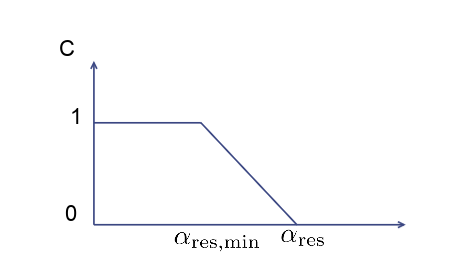
\includegraphics[width=.49\textwidth]{Figure/evanescenceRelaxation.png}
  \caption{Evolution of the coefficient $c$ as a function of $\alpha_{\text{mino}}$.}
  \label{fig:evanescence_relaxation}
\end{figure}

Considering the evolution of the coefficient, the system~\ref{eq:evanescence_relaxation} can be described as follow:
\begin{itemize}
    \item $\alpha_{\text{res}} < \alpha_{\text{mino}}$ : the system is unchanged.
    \item $\alpha_{\text{res,min}} < \alpha_{\text{mino}} < \alpha_{\text{res}}$: partial relaxation of the velocity of the minority phase toward the velocity of the majority phase. The momentum equation solved for the minority phase is a relaxation equation that brings the velocity of the minority phase to that of the majority phase.
    \item $\alpha_{\text{mino}} < \alpha_{\text{res,min}}$: the system is fully reduced by summing the momentum equation of $\alpha_{\text{mino}}$ with $\alpha_{\text{pred}}$. 
\end{itemize}

In other words, when $\alpha$ of the minority phase is less than $\texttt{alpha\_res\_min}$ (i.e., $c=1$), we are in pure HEM, whereas when $\alpha$ of the minority phase is greater than $\texttt{alpha\_res}$, we are in the Two-fluid model. Thus, when we are between the two, we are in a linear combination of the two cases (relaxation) to avoid making the transition abruptly. It should also be noted that in the case of a two-phase system, the minority phase is defined by $\alpha<0.5$. Therefore, if we take $\texttt{alpha\_res}$=1 and $\texttt{alpha\_res\_min}$=0.5 with 2 phases, it means we are always in HEM for the minority phase because $\alpha<0.5$ for the minority phase is always satisfied with 2 phases. However, if we only want to avoid velocity problems with the minority phase when it tends to disappear, we rather impose $\texttt{alpha\_res}=\num{1.e-6}$ (arbitrary pseudo-zero) and $\texttt{alpha\_res\_min}=\num{5.e-7}$ (slightly lower to smooth the transition to HEM), this is ultimately equivalent to having a single-phase system.

This operation is implemented through the object \texttt{correlation}. 
Equation~\ref{eq:evanescence_relaxation} is an example of a correlation that can be used. 
Correlations related to the momentum equations are documented in~\ref{sec:phyical_modeling_drift_velocity} and correlation link to the energy equations are documented in~\ref{sec:phyical_modeling_interface_heat_flux}.

%%%%%%%%%%%%%%%%%%%%%%
\section{Evanescence operator and energy equation\label{sec:evan-ope-and-nrj}}

As reminder, the energy equations for the minority phase reads
\begin{multline}
    \label{eq:eva_energy}
    \frac{\partial \alpha_{\text{mino}} \rho_{\text{mino}} h_{\text{mino}}}{\partial t}+\nabla \cdot\left(\alpha_{\text{mino}} \rho_{\text{mino}} h_{\text{mino}} \vec{v}_{\text{\text{mino}}}\right)=-p\left[\frac{\partial \alpha_{\text{mino}}}{\partial t} +\nabla \cdot\left(\alpha_{\text{mino}} \vec{v}_{\text{mino}}\right)\right] \\
    +\nabla \cdot\left(\alpha_{\text{mino}} \lambda_{\text{mino}} \nabla T_{\text{mino}}\right)+q_{\text{mino,p}}+q_{\text{mino,i}}
\end{multline}
where $q_{\text{mino},i}$ the interfacial flux, $q_{\text{mino},p}$ the parietal flux (to evaluate the diffusive flux near wall boundary conditions). This parietal flux $q_{\text{mino},p}$ can be linked to the mass interface flux $\Gamma_i$ thought a correlation. In this case, they are linked as follow
\begin{equation}
    \Gamma_g = -\Gamma_l = \frac{q_{l} + q_{g}}{L_{\text{vap}}},
\end{equation}
with $L_{\text{vap}}$ the vaporisation enthalpy. For the same reason as mentioned in the previous section, the problem can be ill-posed if the minority phase tends toward zero. For this reason, the evanescence operator can be applied to the energies equations. We obtain the same system than for the momentum one :
\begin{equation}
\label{eq:evanescence_nrj}
\begin{pmatrix}
{\mathcal{E}_{\text{pred}}}  \\
{\mathcal{E}_{\text{mino}}}
\end{pmatrix}
\Longrightarrow
\begin{pmatrix}
{\mathcal{E}_{\text{pred}}} + c {\mathcal{E}_{\text{mino}}} - c \parent{T_{\text{mino}}=T_{\text{pred}}+T_{\text{corr}}} \\
\parent{1 - c} {\mathcal{E}_{\text{mino}}} + c \parent{T_{\text{mino}}=T_{\text{pred}}+T_{\text{corr}}}
\end{pmatrix}
\end{equation}

Similarly to the momentum equation, it is necessary to define a relevant minority phase temperature in the case that $\alpha_{\text{mino}}$ is too low. In this case, it is important to define $T_{\text{mino}}$. Two scenarios may arise:
\begin{description}
    \item[No phase change ($\Gamma_{\text{mino}}=0$):] in this case $q_{\text{mino},i}= h \parent{T_{\text{mino}}-T_{\text{mino,sat}}}$ (with $h$ the heat transfer coefficient) and there is no need of evanescence operator if $h$ does not tend toward zero.
    % 16'
    \item[Considering phase change ($\Gamma_{\text{mino}} \neq 0$):] in this case $q_{\text{mino}} = h \parent{T_{\text{mino}}-T_{\text{mino,sat}}} + \Gamma_{\text{mino}} h_{\text{mino}}$. The term $\Gamma_{\text{mino}} h_{\text{mino}}$ is related to the default of energy due to mass transfer at the interface. It must be noted that if $\Gamma_{\text{mino}} > 0$ then $h_{\text{mino}} = h_{\text{mino,sat}}$. The underlying idea is that the phase is created from an interface at saturation temperature. This specificity is well documented in CATHARE documentation~\cite{dummycitation}. It aims at avoiding that vapour condensate considering too low latent heat and stay to high. 
\end{description}
It has to be precised that $T_{\text{mino}}$ can be imposed at $T_{\text{sat}}$ if the composite medium is at saturation.
% Il y a dissymétrie ici. Le traitement spécifique de h en fonction du signe de $\Gamma_k$ est pensé de façon à ce que la vapeur soit la phase minoritaire. Vérifier ça avec Antoine ou Corentin.


%%%%%%%%%%%%%%%%%%%%%%
\section{Flux limiter\label{sec:flux-limiter}} %19'

%First thermodynamic principle at resolved scales:
%\begin{equation}
%    \Gamma_{k} L_v = [ \lambda \nabla T] \; .
%\end{equation}
The source term $\Gamma_{k}$ has to respect two conditions:
\begin{enumerate}
    \item flux consistency: $q_{k i} + q_{k i} =0$
    \item positive volume fractions for each phase: $\alpha_i(\boldsymbol{x},t) \; \forall \; \boldsymbol{x} \; \textrm{and} \ t $. 
\end{enumerate}
To achieve this goal, a first estimation of the interfacial heat flux is calculated from correlations for each phase:
\begin{equation}
    \label{eq:evanescence_clipping}
    \Gamma_{k} = f(q_{i}) \; \text{such as} \; q_{\text{mino}} + q_{\text{pred}} = 0.
\end{equation}
Then a flux limiter is calculated from the transport equation of the minority phase:
\begin{equation}
    \label{eq:evanescence_Glim}
    \Gamma_{\text{lim}}=\nabla \cdot (\alpha_{\text{mino}}\rho_{\text{mino}})\overrightarrow{v}_{\text{mino}}-\frac{\partial \alpha_{\text{mino}}\rho_{\text{mino}}}{\partial t}.
\end{equation}
If $\Gamma_{k} < \Gamma_{\text{lim}}$ both conditions are respected. 

However, if $\Gamma_{k} \geq \Gamma_{\text{lim}}$, the resulting volume fraction of the minority phase would be negative. 
In this case, $\Gamma_{k}$ is imposed at $\Gamma_{\text{lim}}$ value and the flux consistence is imposed through the following relations
\begin{align}
    q_{\text{mino}} &= h \left( T_{\text{mino}}-T_{\textrm{mino,sat}} \right) + \Gamma_{\text{lim}} h_{\text{mino}},\\
    q_{\text{pred}} &= -q_{\text{mino}}.
\end{align}
These operations are coded in file \texttt{Source\_Flux\_interfacial\_base}.

%%%%%%%%%%%%%%%%%%%%%%
\section{Dataset\label{sec:eva-dataset}}

An example of evanescence operator is 
\begin{lstlisting}[caption={data set definition},captionpos=b,escapechar=|]
    QDM_Multiphase
    {
        evanescence { homogene { alpha_res 1.e-6 alpha_res_min 5.e-7 } }
        solveur_pression petsc cli_quiet { -pc_type hypre -pc_hypre_type boomeramg -ksp_type fgmres }
        convection { amont }
        diffusion  { turbulente $diffusion { sigma 1 } }
        initial_conditions
        {
            ...
        }
        conditions_limites
        {
            ...
        }
    }
\end{lstlisting}
with \texttt{alpha\_res} corresponding to $\alpha_{\textrm{min}}$ and \texttt{alpha\_res\_min} corresponding to $\alpha_{\textrm{res,min}}$.


%%%%%%%%%%%%%%%%%%%%%%
\section{Coding\label{eva:coding}}

\subsection{Faces}
\begin{itemize}
    \item[\small \textcolor{blue}{\ding{109}}]\texttt{Op\_Evanescence\_Homogene\_Face\_base}: management for faces (linked to momentum equation and so can impose the drift velocity) 
\end{itemize}
The model is implemented in 2 files.
\begin{lstlisting}[language=c++]
void Op_Evanescence_Homogene_Elem_base::readOn(Entree& is)
{
  Param param(que_suis_je());
  param.ajouter("alpha_res", &alpha_res_, Param::REQUIRED);
  param.ajouter("alpha_res_min", &alpha_res_min_);
  param.lire_avec_accolades_depuis(is);
  return is;
}
\end{lstlisting}

\subsection{Elements}

\begin{itemize}
    \item[\small \textcolor{blue}{\ding{109}}]\texttt{Op\_Evanescence\_Homogene\_Elem\_base}: management for elements (linked to mass and energy equations and can weakly imposed conditions for temperature and void fraction, based on fluxes)
\end{itemize}
\begin{lstlisting}[language=c++]
void Op_Evanescence_Homogene_Face_base::readOn(Entree& is)
{
  Param param(que_suis_je());
  param.ajouter("alpha_res", &alpha_res_, Param::REQUIRED);
  param.ajouter("alpha_res_min", &alpha_res_min_);
  param.lire_avec_accolades_depuis(is);

  Pb_Multiphase& pbm = ref_cast(Pb_Multiphase, equation().probleme());
  if (pbm.has_correlation("Vitesse_relative") && !pbm.has_correlation("gravite")) Process::exit(que_suis_je() + " : you must define a multiphase gravity field if you want a drift flux!!");
  if (pbm.has_correlation("Vitesse_relative") && ref_cast(Vitesse_relative_base, pbm.get_correlation("Vitesse_relative").valeur()).needs_vort()) pbm.creer_champ("vorticite");

  return is;
}
\end{lstlisting}

Default values : \texttt{alpha\_res\_} = 0, \texttt{alpha\_res\_min\_} = 0.

\subsection{Implementation}

The model is called for each dimensioning and assembly of blocks or matrices (\texttt{assembler\_blocs}, \texttt{dimensionner\_forblocs}, \texttt{dimensionner\_matrice}). 
It allows adding the equation of the residual phase to the majority phase, locally according to a global criterion \texttt{alpha\_res\_}. 
It is possible to impose an algebraic relationship for velocity and temperature (i.e., $v_l = v_g$ or $v_l = v_g + v_r$ for velocity, $T_l = T_{\text{sat}}$ or $T_l = T_g$ for temperature). 
Conditions on void fraction and temperature are imposed through flux corrections in the mass and energy equations. 
For example, for mass equation:
\begin{equation}
\Gamma_{k,\text{mino}}=\nabla \cdot (\alpha_k\rho_k)\overrightarrow{v_k} - \frac{\partial \alpha_k\rho_k}{\partial t}
\end{equation}
In the case of the energy equation, if the flux is imposed by a correlation, then it is the pressure term that is corrected.

It is implemented as:
\begin{itemize}
\item[\small \textcolor{blue}{\ding{109}}]For elements and faces \texttt{secmem(e, k)} adds corrected flux in right hand side of the equation of local main phase,
\item[\small \textcolor{blue}{\ding{109}}]For elements and faces \texttt{secmem(e, n)} corrects the flux in right hand side of the equation of local evanescent phase,
\item[\small \textcolor{blue}{\ding{109}}]For faces, if a drift velocity model is defined with \texttt{correlation\_vd}, we impose the relative velocity between the local main phase and the local evanescent phase,
\end{itemize}
with \texttt{e} elements, \texttt{k} majority local phase, \texttt{n} evanescent local phase.

%%%%%%%%%%%%%%%%%%%%%%
%\section{Pb_Multiphase_HEM}
%The keyword $Pb\_ Multiphase\_ HEM$ enables the use of a HEM model through $Pb\_ multiphase$. It allows the resolution of $2$ phases mechanicaly and thermally coupled with one common set of equations (mass, momentum and energy). It notably uses $Evanescence\_ Homogene$ to achieve this. It is equivalent to the following line in the data set :
%\begin{lstlisting}[language=c++]
%evanescence { homogene { alpha_res 1 alpha_res_min 0.5 } }
%\end{lstlisting}
%If this keyword is used, it is mandatory to associate an interfacial flux correlation with constant coefficient.
